% This code generated the histograms illustration. We ship the output (converted to SVG)
% directly in order to avoid latex + pdf2svg converter dependencies. When updating this
% code, you should locally regenerate the output and replace the old one with it. Except
% for the pure tikz logic, the code was generated by sphinxcontrib.tikz.

\documentclass[12pt,tikz,border={5pt 0pt 5pt 0pt}]{standalone}
\usepackage[utf8]{inputenc}
\usepackage{amsmath}
\usepackage{pgfplots}
\usetikzlibrary{}
\pagestyle{empty}
\definecolor{myorange}{RGB}{254,128,16}
\definecolor{mygreen}{RGB}{47,161,46}
\begin{document}
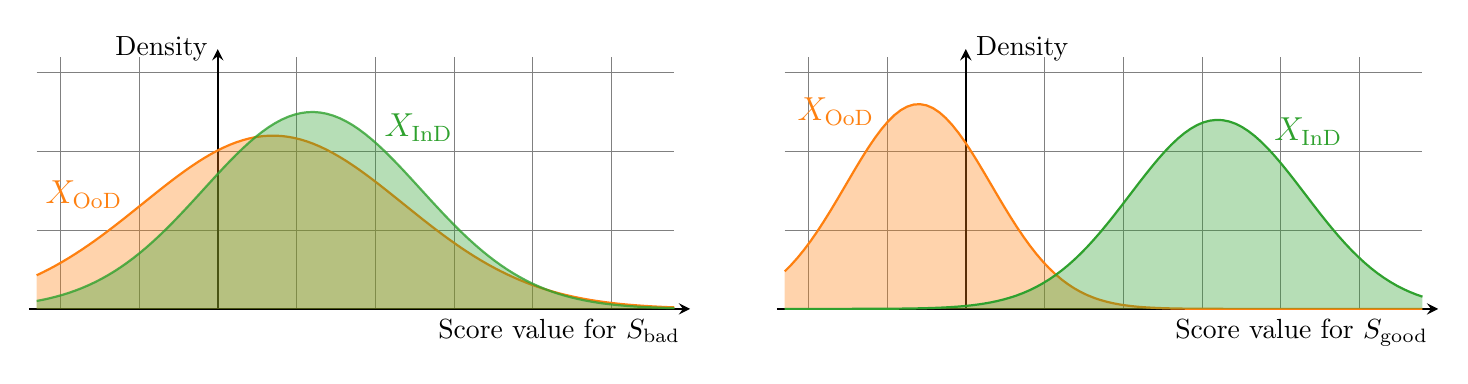
\begin{tikzpicture}[domain=-2.3:5.8, samples=100]
  \begin{scope}
    \draw[very thin,color=gray] (-2.3, 0) grid (5.8, 3.2);
    \draw[thick, -stealth] (-2.4, 0) -- (6, 0) node[below left] {Score value for $S_{\text{bad}}$};
    \draw[thick, -stealth] (0, 0) -- (0, 3.3) node[left] {Density};
    \fill[color=myorange, fill opacity=.35] (-2.3, 0) -- plot (\x, {2.2*1.2^(-(\x -.7)*(\x -.7)}) -- (5.8, 0);
    \draw[color=myorange, thick] plot (\x, {2.2*1.2^(-(\x -.7)*(\x -.7)});
    \draw[color=myorange] (-1.7, 1.45) node {\large $X_{\text{\normalfont OoD}}$};
    \fill[color=mygreen, fill opacity=.35] (-2.3, 0) -- plot (\x, {2.5*1.3^(-(\x -1.2)*(\x -1.2)}) -- (5.8, 0);
    \draw[color=mygreen, opacity=.8, thick] plot (\x, {2.5*1.3^(-(\x -1.2)*(\x -1.2)});
    \draw[color=mygreen] (2.55, 2.3) node {\large $X_{\text{\normalfont InD}}$};
  \end{scope}
  \begin{scope}[xshift=9.5cm]
    \draw[very thin,color=gray] (-2.3, 0) grid (5.8, 3.2);
    \draw[thick, -stealth] (-2.4, 0) -- (6, 0) node[below left] {Score value for $S_{\text{good}}$};
    \draw[thick, -stealth] (0, 0) -- (0, 3.3) node[right] {Density};
    \fill[color=myorange, fill opacity=.35] (-2.3, 0) -- plot (\x, {2.6*1.8^(-(\x +.6)*(\x +.6)}) -- (5.8, 0);
    \draw[color=myorange, thick] plot (\x, {2.6*1.8^(-(\x +.6)*(\x +.6)});
    \draw[color=myorange] (-1.65, 2.5) node {\large $X_{\text{\normalfont OoD}}$};
    \fill[color=mygreen, fill opacity=.35] (-2.3, 0) -- plot (\x, {2.4*1.5^(-(\x -3.2)*(\x -3.2)}) -- (5.8, 0);
    \draw[color=mygreen, thick] plot (\x, {2.4*1.5^(-(\x -3.2)*(\x -3.2)});
    \draw[color=mygreen] (4.35, 2.25) node {\large $X_{\text{\normalfont InD}}$};
  \end{scope}
\end{tikzpicture}
\end{document}
